\documentclass{beamer}
\usepackage[utf8]{inputenc}
\usepackage[spanish]{babel}
\usepackage{amsfonts,amsmath,amssymb}
\usepackage{booktabs}
\usepackage{graphicx}
\usepackage{multirow}
\usepackage{array}
\usetheme{sintef}
\usepackage{orcidlink}

\newcommand{\testcolor}[1]{\colorbox{#1}{\textcolor{#1}{test}}~\texttt{#1}}
\usefonttheme[onlymath]{serif}

\titlebackground*{assets/UNIbackground}

\newcommand{\hrefcol}[2]{\textcolor{cyan}{\href{#1}{#2}}}

\title[BRIEF: Binary Robust Independent Elementary Features]{\textbf{BRIEF: Binary Robust Independent Elementary Features}}
\subtitle{MIA-301 Visión por Computadora\\ Escuela de Posgrado  FIIS - UNI}
\course{Maestría en Inteligencia Artificial\vspace{0.2cm}}
\author
    {
        Andrés Flores B. \orcidlink{0009-0008-6960-0852} \and
        Víctor Lazo P. \orcidlink{0000-0002-3293-6415} \and
        Rubén López M. \orcidlink{0009-0004-5446-086X} \and
        Juan Quispe H. \orcidlink{0000-0003-3957-5728}
    }

\date{\vspace{0.2cm}21 de octubre de 2026}

\begin{document}

\maketitle

% ==============================================================================
% SLIDE 2: AGENDA (20 MINUTOS)
% ==============================================================================
\begin{frame}{Estructura de la Presentación}
\framesubtitle{}
\begin{columns}[T]
\begin{column}{0.48\textwidth}
\begin{colorblock}[black]{sintefgrey}{1. Descripción general del método}
\scriptsize
\begin{itemize}\setlength{\itemsep}{2pt}
    \item Motivación científica y limitaciones de SIFT/SURF.
    \item Formulación matemática de las pruebas $\tau(\mathbf{p};\mathbf{x},\mathbf{y})$.
    \item Pre-suavizado Gaussiano y geometrías ($G_I \dots G_V$).
    \item Distribuciones estadísticas en el espacio de Hamming.
\end{itemize}
\end{colorblock}
\vspace{0.15cm}
\begin{colorblock}[black]{sintefgrey}{2. Escala e Invariancia de rotacion}
\scriptsize
\begin{itemize}\setlength{\itemsep}{2pt}
    \item Robustez e invarianza a cambios de escala y rotación.
    \item Análisis de \texttt{O-BRIEF} y detectores (\texttt{CenSurE}, \texttt{FAST}).
    \item Comparación con SIFT, SURF, U-SURF, ORB y BRISK.
\end{itemize}
\end{colorblock}
\end{column}
\begin{column}{0.48\textwidth}
\begin{colorblock}[black]{sintefgrey}{3. Aplicaciones}
\scriptsize
\begin{itemize}\setlength{\itemsep}{2pt}
    \item Visual SLAM y odometría en robótica móvil.
    \item Realidad aumentada en dispositivos con IMU.
    \item Localización e indexación 3D a gran escala.
\end{itemize}
\end{colorblock}
\vspace{0.15cm}
\begin{colorblock}[black]{sintefgrey}{4. Ventajas y limitaciones}
\scriptsize
\begin{itemize}\setlength{\itemsep}{2pt}
    \item Aceleración 35$\times$--41$\times$ e instrucción \texttt{POPCNT}.
    \item Limitaciones geométricas y fotométricas.
    \item Conclusiones, referencias y legado científico.
\end{itemize}
\end{colorblock}
\end{column}
\end{columns}
\end{frame}

% ==============================================================================
% SECCIÓN 1: METHOD OVERVIEW
% ==============================================================================
\section{Descripción general del método}

\begin{chapter}[assets/UNIbackground_negative]{maincolor}{1. Descripción general del método}
\footnotesize
\begin{itemize}
    \item Paradigma de descripción binaria directa sobre parches suavizados
    \item Formulación matemática, kernels de suavizado y muestreo espacial
    \item Emparejamiento ultrarrápido mediante distancia de Hamming
\end{itemize}
\end{chapter}

\footlinecolor{maincolor}
\footlinepayoff{Grupo 04 (FIIS-UNI) $\vert$ BRIEF (Calonder et al., ECCV 2010)}

\begin{frame}{Motivación Científica y Estado del Arte Previo}
\framesubtitle{¿Por qué reemplazar descriptores de punto flotante por cadenas binarias?}
\begin{columns}[T]
\begin{column}{0.53\textwidth}
\scriptsize
\textbf{Limitaciones de los descriptores clásicos:}
\begin{itemize}\setlength{\itemsep}{4pt}
    \item \textbf{SIFT} (Lowe, 2004): vector de $128$ flotantes ($512$ bytes/punto). Altamente discriminativo, pero costoso en extracción y búsqueda ($\mathcal{O}(d)$ en norma $L_2$).
    \item \textbf{SURF-64} (Bay et al., 2008): $64$ flotantes ($256$ bytes/punto) con imágenes integrales, pero aún elevado en memoria para millones de puntos.
    \item \textbf{Compresión a posteriori} (PCA, LDA, Cuantización, LSH): obligan a \emph{calcular primero el descriptor flotante completo} antes de binarizarlo o reducirlo.
\end{itemize}
\end{column}
\begin{column}{0.44\textwidth}
\begin{colorblock}[black]{sinteflightgreen}{Propuesta de BRIEF (Calonder et al., 2010)}
\scriptsize
Omitir el cálculo de histogramas de gradientes construyendo \textbf{directamente una cadena binaria} a partir de comparaciones de intensidad de pares de píxeles, \textbf{sin fase de entrenamiento} (a diferencia de \emph{Random Ferns} o árboles aleatorios).
\end{colorblock}
\vspace{0.1cm}
\centering
\scriptsize
\begin{tabular}{lcc}
\toprule
\textbf{Descriptor} & \textbf{Dimensión} & \textbf{Memoria} \\
\midrule
SIFT & 128 floats & 512 B \\
SURF-64 & 64 floats & 256 B \\
\textbf{BRIEF-64} & \textbf{512 bits} & \textbf{64 B} \\
\textbf{BRIEF-32} & \textbf{256 bits} & \textbf{32 B} \\
\textbf{BRIEF-16} & \textbf{128 bits} & \textbf{16 B} \\
\bottomrule
\end{tabular}
\end{column}
\end{columns}
\end{frame}

\begin{frame}{Kernels de Pre-Suavizado Gaussiano}
\framesubtitle{Reducción de la sensibilidad al ruido de alta frecuencia}
\begin{columns}[T]
\begin{column}{0.44\textwidth}
\scriptsize
\begin{itemize}\setlength{\itemsep}{4pt}
    \item \textbf{Interpretación diferencial:} La comparación $\mathbf{p}(\mathbf{x}) < \mathbf{p}(\mathbf{y})$ evalúa el \emph{signo de la derivada direccional} a lo largo de $\mathbf{y} - \mathbf{x}$.
    \item Evaluar píxeles individuales sin filtrar hace que el descriptor sea muy sensible al ruido electrónico y al aliasing.
    \item \textbf{Parámetro óptimo del paper:} Convolución previa con un kernel Gaussiano discreto de ventana $9 \times 9$ y $\sigma \in [1, 3]$ ($\sigma = 2.0$ en todos los experimentos).
    \item En la secuencia \texttt{Wall}, el suavizado incrementa hasta $+18\%$ la tasa de reconocimiento en pares difíciles (\texttt{Wall 1|4} a \texttt{1|6}).
\end{itemize}
\end{column}
\begin{column}{0.54\textwidth}
\centering
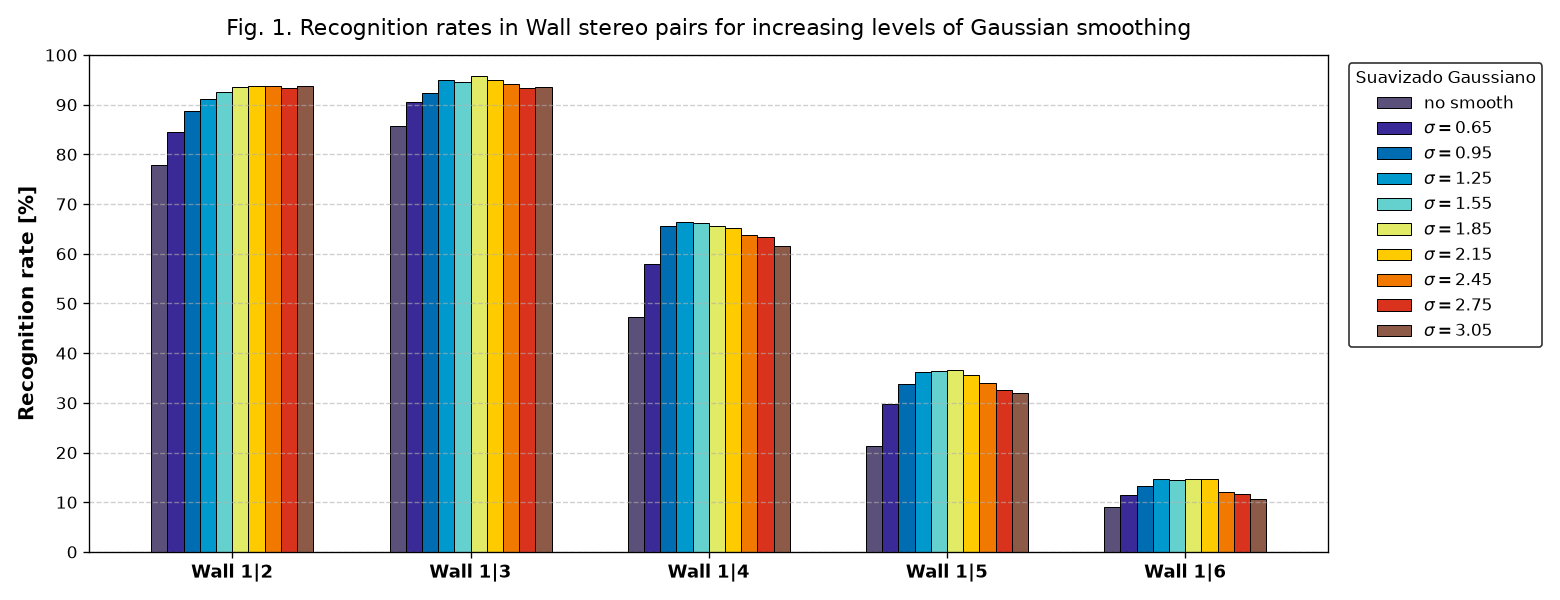
\includegraphics[width=0.98\textwidth]{assets/fig1_smoothing.png}
\tiny \textbf{Fig. 1 reproducida:} Tasa de reconocimiento en \texttt{Wall} para 10 niveles de suavizado Gaussiano ($\sigma \in [0, 3.05]$, $n_d=512$, $G_{II}$).
\end{column}
\end{columns}
\end{frame}


\begin{frame}{Explicación del Método BRIEF}
\framesubtitle{Pruebas Elementales de Intensidad y Construcción del Bitstring}
\scriptsize
Sea $\mathbf{p}$ un parche de imagen de tamaño $S \times S$ centrado en un punto de interés (por defecto $S = 31$ píxeles):
\begin{columns}[T]
\begin{column}{0.48\textwidth}
\begin{colorblock}[black]{sintefgrey}{1. Prueba Binaria Elemental (Ec. 1)}
\scriptsize
Se define la prueba $\tau$ sobre un par de ubicaciones $(\mathbf{x}, \mathbf{y})$ dentro del parche suavizado:
\begin{equation*}
\tau(\mathbf{p}; \mathbf{x}, \mathbf{y}) :=
\begin{cases}
1 & \text{si } \mathbf{p}(\mathbf{x}) < \mathbf{p}(\mathbf{y}) \\
0 & \text{en otro caso}
\end{cases}
\end{equation*}
donde $\mathbf{p}(\mathbf{x})$ es la intensidad suavizada en $\mathbf{x} = (u, v)^\top$.
\end{colorblock}
\end{column}
\begin{column}{0.48\textwidth}
\begin{colorblock}[black]{sintefgrey}{2. Descriptor Binario BRIEF-$k$ (Ec. 2)}
\scriptsize
Para un conjunto de $n_d$ pares $\{(\mathbf{x}_i, \mathbf{y}_i)\}_{i=1}^{n_d}$, el descriptor es la cadena de $n_d$ bits ($k = n_d/8$ bytes):
\begin{equation*}
f_{n_d}(\mathbf{p}) := \sum_{1 \le i \le n_d} 2^{i-1}\,\tau(\mathbf{p}; \mathbf{x}_i, \mathbf{y}_i)
\end{equation*}
Con $n_d \in \{128, 256, 512\}$ (\texttt{BRIEF-16}, \texttt{BRIEF-32}, \texttt{BRIEF-64}).
\end{colorblock}
\end{column}
\end{columns}
\vspace{0.15cm}
\begin{itemize}
    \item \textbf{Métrica de similitud (Distancia de Hamming):} Número de bits diferentes evaluado mediante instrucción lógica \texttt{XOR} seguida de conteo de bits en hardware (\texttt{POPCNT} en SSE4.2):
    \[
        d_H\big(f_{n_d}(\mathbf{p}), f_{n_d}(\mathbf{q})\big) = \operatorname{POPCNT}\!\big(f_{n_d}(\mathbf{p}) \oplus f_{n_d}(\mathbf{q})\big)
    \]
\end{itemize}
\end{frame}



\begin{frame}{Disposición Espacial de las Pruebas Binarias}
\framesubtitle{Cinco geometrías estocásticas y deterministas de muestreo ($G_I \dots G_V$)}
\scriptsize
Asumiendo el origen $(0,0)^\top$ en el centro del parche de tamaño $S \times S$ ($S=31$):
\begin{itemize}\setlength{\itemsep}{1.5pt}
    \item \textbf{$G_I$ (Uniforme i.i.d.):} $(\mathbf{X}, \mathbf{Y}) \sim \text{i.i.d. }\mathcal{U}\!\left(-\frac{S}{2}, \frac{S}{2}\right)$. Cobertura uniforme hasta los bordes del parche.
    \item \textbf{$G_{II}$ (Gaussiana Isotrópica i.i.d.):} $(\mathbf{X}, \mathbf{Y}) \sim \text{i.i.d. }\mathcal{N}\!\left(0, \frac{1}{25}S^2\right) \iff \sigma = \frac{S}{5}$. Mayor densidad cerca del centroide.
    \item \textbf{$G_{III}$ (Gaussiana Local en 2 pasos):} $\mathbf{X} \sim \mathcal{N}\!\left(0, \frac{1}{25}S^2\right)$ y $\mathbf{Y} \sim \mathcal{N}\!\left(\mathbf{x}_i, \frac{1}{100}S^2\right)$. Pruebas más locales alrededor de $\mathbf{x}_i$.
    \item \textbf{$G_{IV}$ (Grilla Polar Aleatoria):} $(\mathbf{x}_i, \mathbf{y}_i)$ muestreados aleatoriamente sobre ubicaciones discretas de una grilla polar gruesa.
    \item \textbf{$G_V$ (Grilla Polar Determinista):} $\forall i: \mathbf{x}_i = (0,0)^\top$ e $\mathbf{y}_i$ recorre todos los nodos de la grilla polar ($n_d$ puntos).
\end{itemize}
\vspace{0.05cm}
\centering
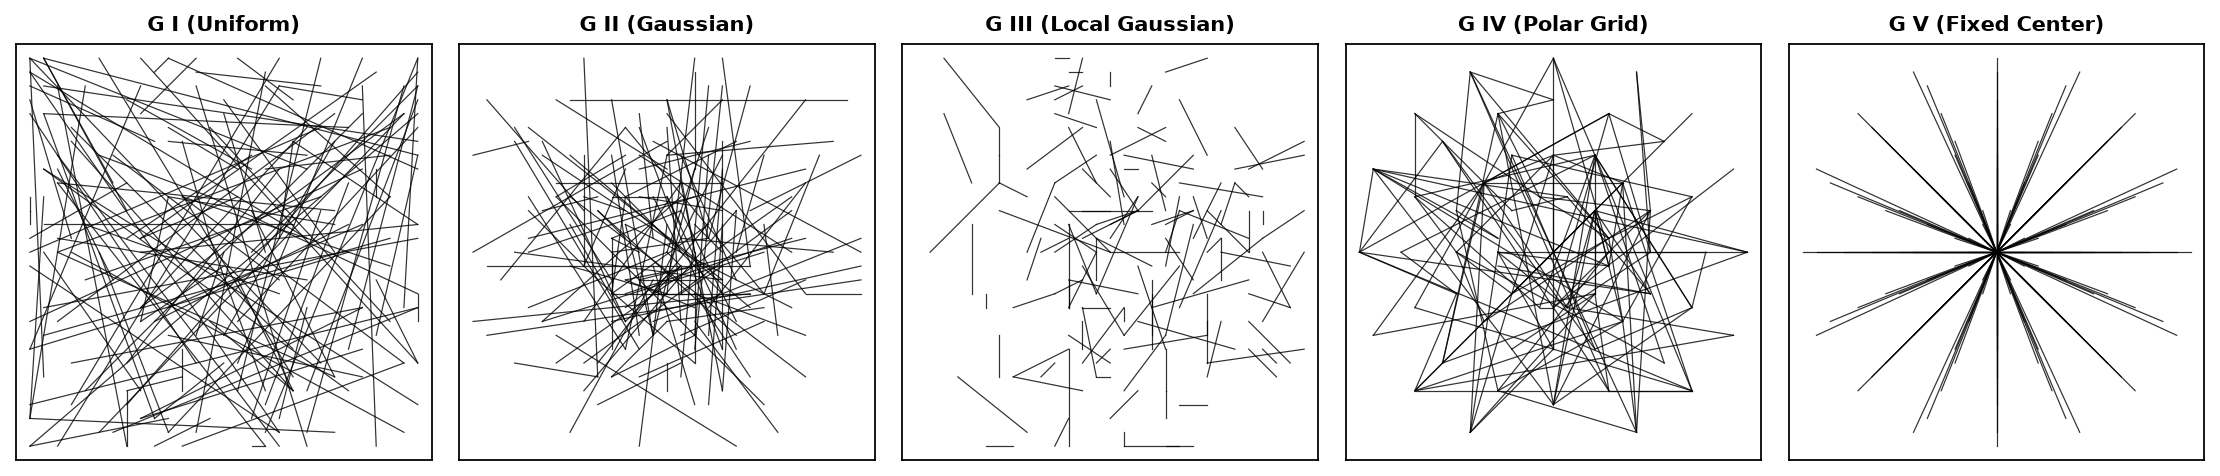
\includegraphics[width=0.90\textwidth]{assets/fig2_geometries.png}
\end{frame}

\begin{frame}{Evaluación de Geometrías y Distribuciones de Distancia}
\framesubtitle{Superioridad de los diseños aleatorios ($G_I$--$G_{IV}$) y separabilidad en el espacio de Hamming}
\begin{columns}[T]
\begin{column}{0.45\textwidth}
\centering
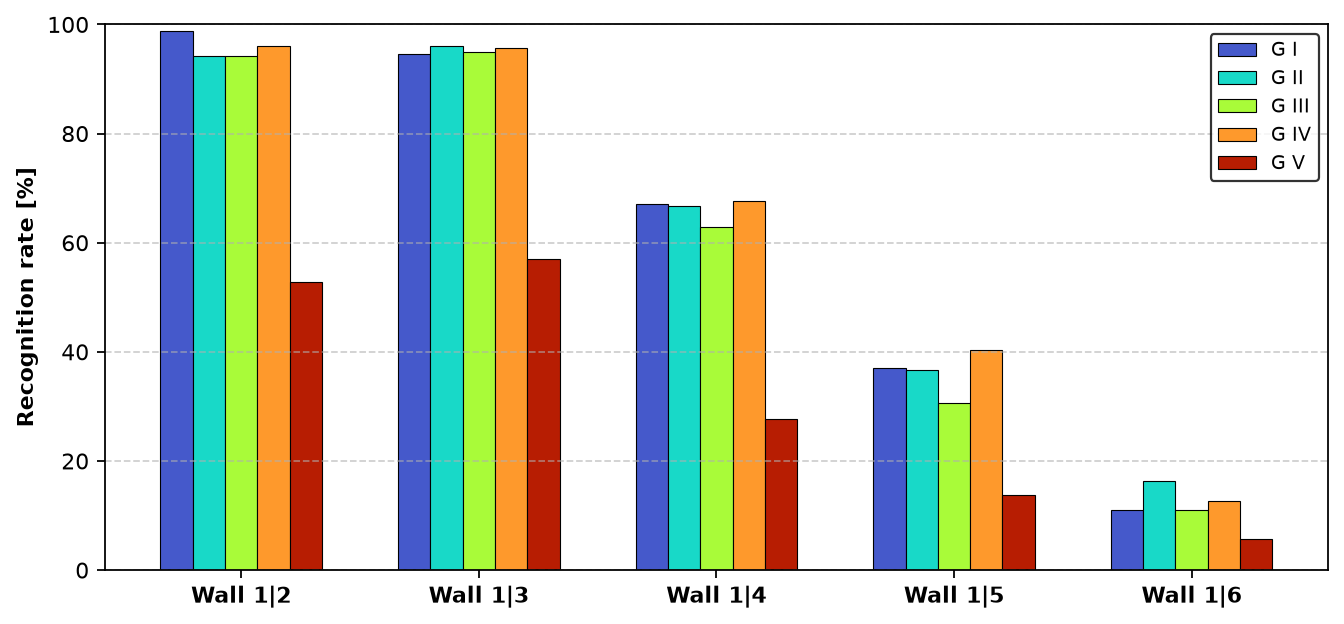
\includegraphics[width=0.92\textwidth]{assets/fig3_rates.png}
\scriptsize
\begin{itemize}\setlength{\itemsep}{2pt}
    \item La estrategia simétrica $G_V$ pierde frente a todos los diseños aleatorios $G_I \dots G_{IV}$.
    \item \textbf{$G_{II}$ (Gaussiana)} logra una ventaja consistente y se adopta en el resto del paper.
\end{itemize}
\end{column}
\begin{column}{0.53\textwidth}
\centering
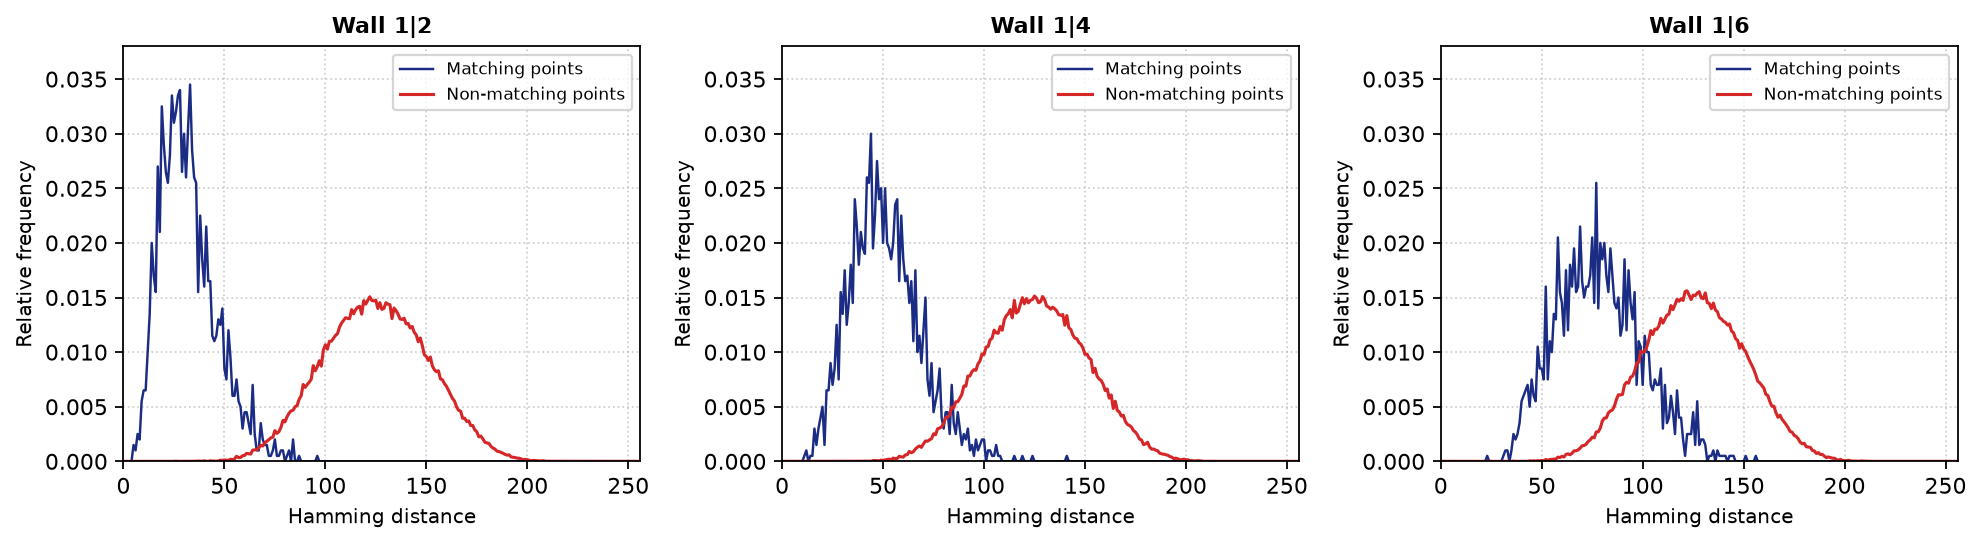
\includegraphics[width=0.98\textwidth]{assets/fig4_distributions.png}
\scriptsize
\begin{itemize}\setlength{\itemsep}{2pt}
    \item \textbf{Non-matching (rojo):} Campana Gaussiana centrada en $n_d/2 = 128$ bits ($32 \times 8 = 256$ bits).
    \item \textbf{Matching (azul):} Media baja ($\sim 32.7$ bits en \texttt{Wall 1|2}) que crece con el ángulo de cámara ($\sim 79.0$ bits en \texttt{1|6}).
    \item La clara separación entre ambas curvas maximiza la tasa de acierto del clasificador 1-NN.
\end{itemize}
\end{column}
\end{columns}
\end{frame}

% ==============================================================================
% SECCIÓN 2: SCALE AND ROTATION INVARIANCE
% ==============================================================================
\section{Escala e invariancia de rotación}

\begin{chapter}[assets/UNIbackground_negative]{sintefdarkgreen}{2. Escala e invariancia de rotación}
\footnotesize
\begin{itemize}
    \item Análisis de invarianza a cambios de escala y rotación en plano
    \item El costo de la invarianza a orientación: BRIEF vs.\ U-SURF vs.\ SURF vs.\ O-BRIEF
    \item Comparación estructural y experimental con otros detectores y descriptores
\end{itemize}
\end{chapter}

\footlinecolor{sintefdarkgreen}
\footlinepayoff{Grupo 04 (FIIS-UNI) $\vert$ BRIEF (Calonder et al., ECCV 2010)}

\begin{frame}{Rotación en BRIEF} 
\framesubtitle{}
\begin{center} 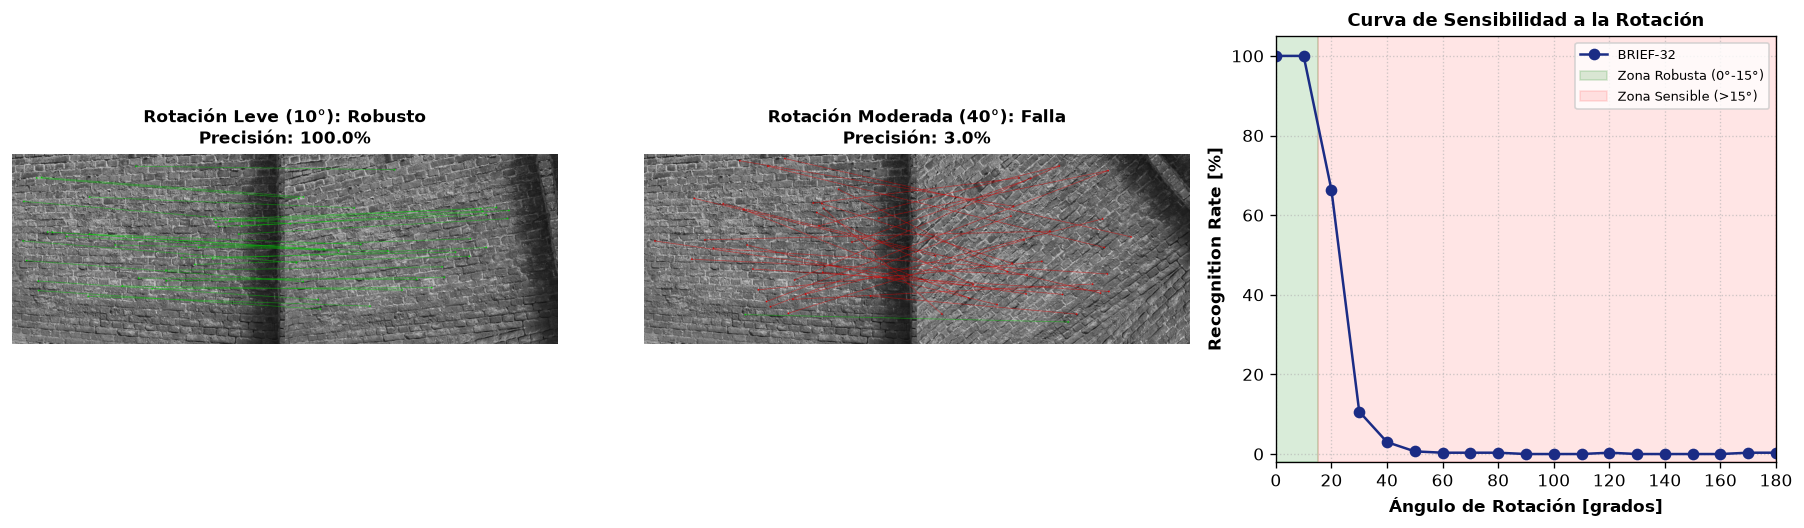
\includegraphics[width=1\textwidth]{BRIEF_G04_MIA_09_SEC_B/images/rotacion.png} 
\end{center} 
\end{frame}

\begin{frame}{Escala en BRIEF} 
\framesubtitle{}
\begin{center} 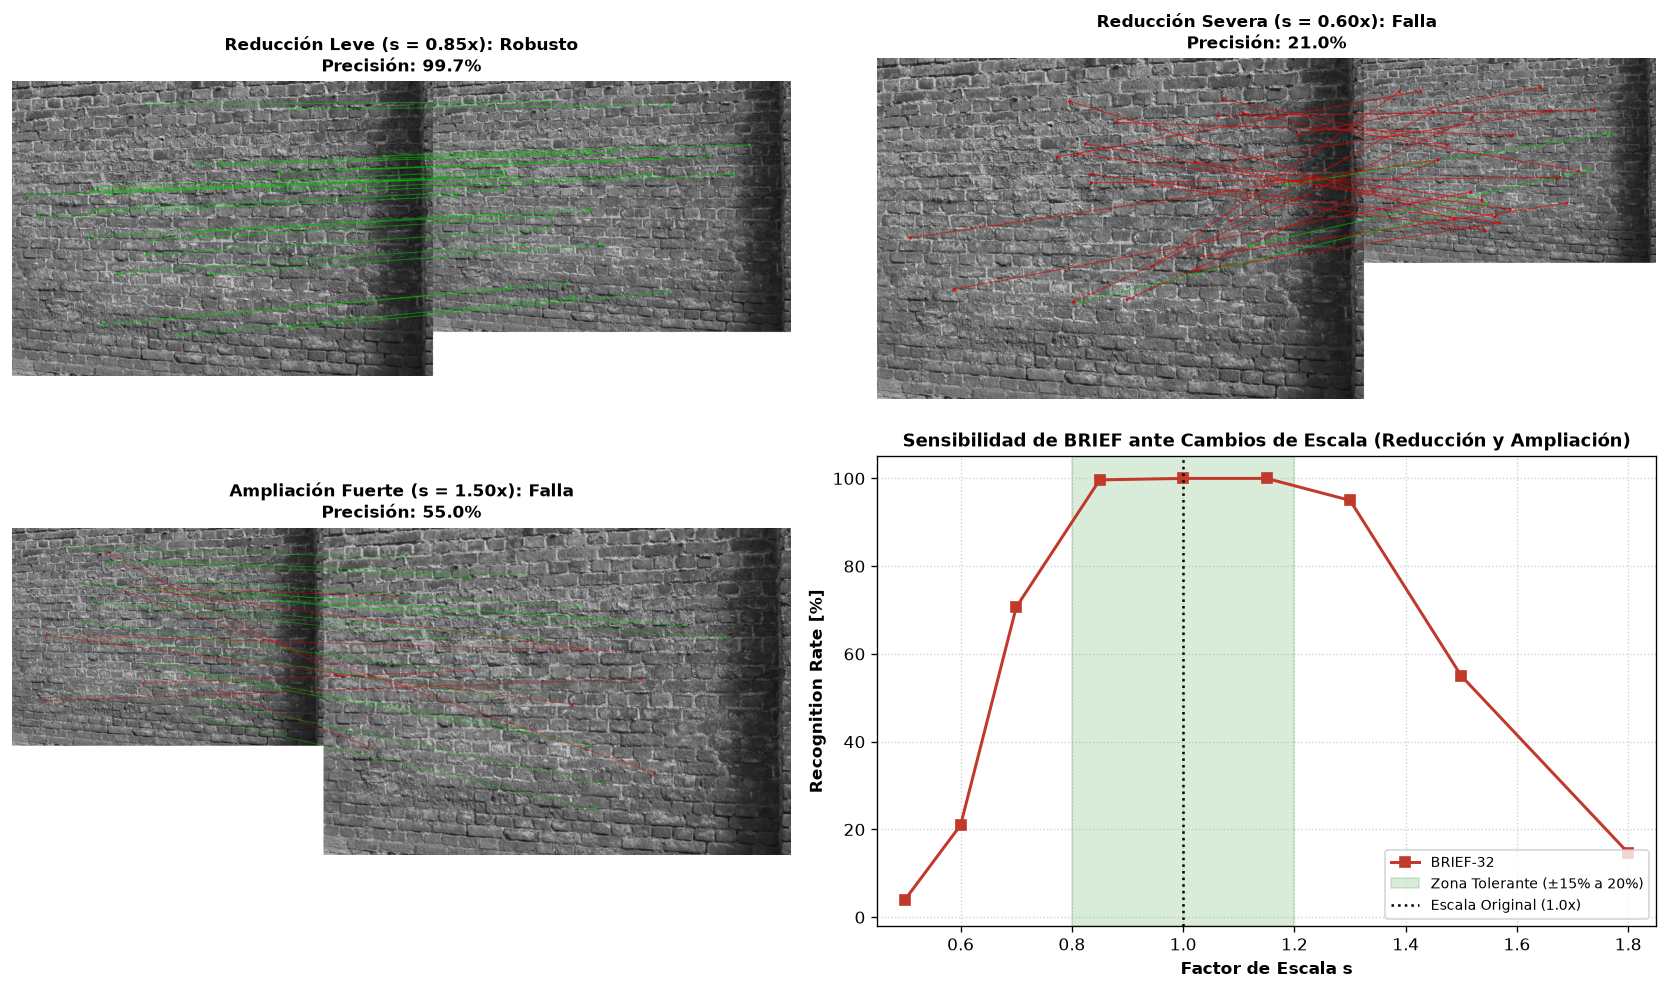
\includegraphics[width=0.75\textwidth]{BRIEF_G04_MIA_09_SEC_B/images/escala.png} 
\end{center} 
\end{frame}

\begin{frame}{Análisis de Invarianza a Escala y Rotación en BRIEF}
\framesubtitle{¿Es BRIEF invariante o robusto ante transformaciones geométricas?}
\begin{columns}[T]
\begin{column}{0.48\textwidth}
\begin{colorblock}[black]{sintefgrey}{Invarianza a la Escala}
\scriptsize
\begin{itemize}\setlength{\itemsep}{3pt}
    \item \textbf{No es invariante a la escala por diseño:} Opera sobre un parche fijo $S \times S$ en la imagen sin construir una pirámide espacio-escala.
    \item \textbf{Robustez moderada:} El pre-suavizado Gaussiano ($\sigma = 2.0$) y el muestreo isotrópico $G_{II}$ le otorgan tolerancia a cambios moderados de escala y perspectiva (secuencias \texttt{Wall} y \texttt{Fountain}).
    \item \textbf{Integración con detectores multi-escala:} Acoplado con detectores rápidos como \textbf{CenSurE / STAR} (Agrawal et al., 2008) o pirámides FAST (como en \textbf{ORB}), adquiere adaptabilidad multi-escala.
\end{itemize}
\end{colorblock}
\end{column}
\begin{column}{0.48\textwidth}
\begin{colorblock}[black]{sintefgrey}{Invarianza a la Rotación}
\scriptsize
\begin{itemize}\setlength{\itemsep}{3pt}
    \item \textbf{No está diseñado para invarianza rotacional:} Los pares $(\mathbf{x}_i, \mathbf{y}_i)$ tienen orientación fija respecto a los ejes de la imagen.
    \item \textbf{Alta robustez entre $0^\circ$ y $15^\circ$:} Presenta degradación mínima hasta $10^\circ\text{--}15^\circ$ (superior a SURF-64 e igual a U-SURF-64), seguida de una caída pronunciada para $>25^\circ$.
    \item \textbf{Principio demostrado en el paper:} Lograr invarianza a orientación conlleva un costo tanto en velocidad como en tasa de reconocimiento cuando la rotación real es pequeña.
\end{itemize}
\end{colorblock}
\end{column}
\end{columns}
\end{frame}

\begin{frame}{Influencia del Detector y Sensibilidad a la Rotación}
\framesubtitle{Experimentos de la Figura 9: Detectores CenSurE vs.\ SURF y Rotación $0^\circ \dots 180^\circ$}
\begin{columns}[T]
\begin{column}{0.55\textwidth}
\centering
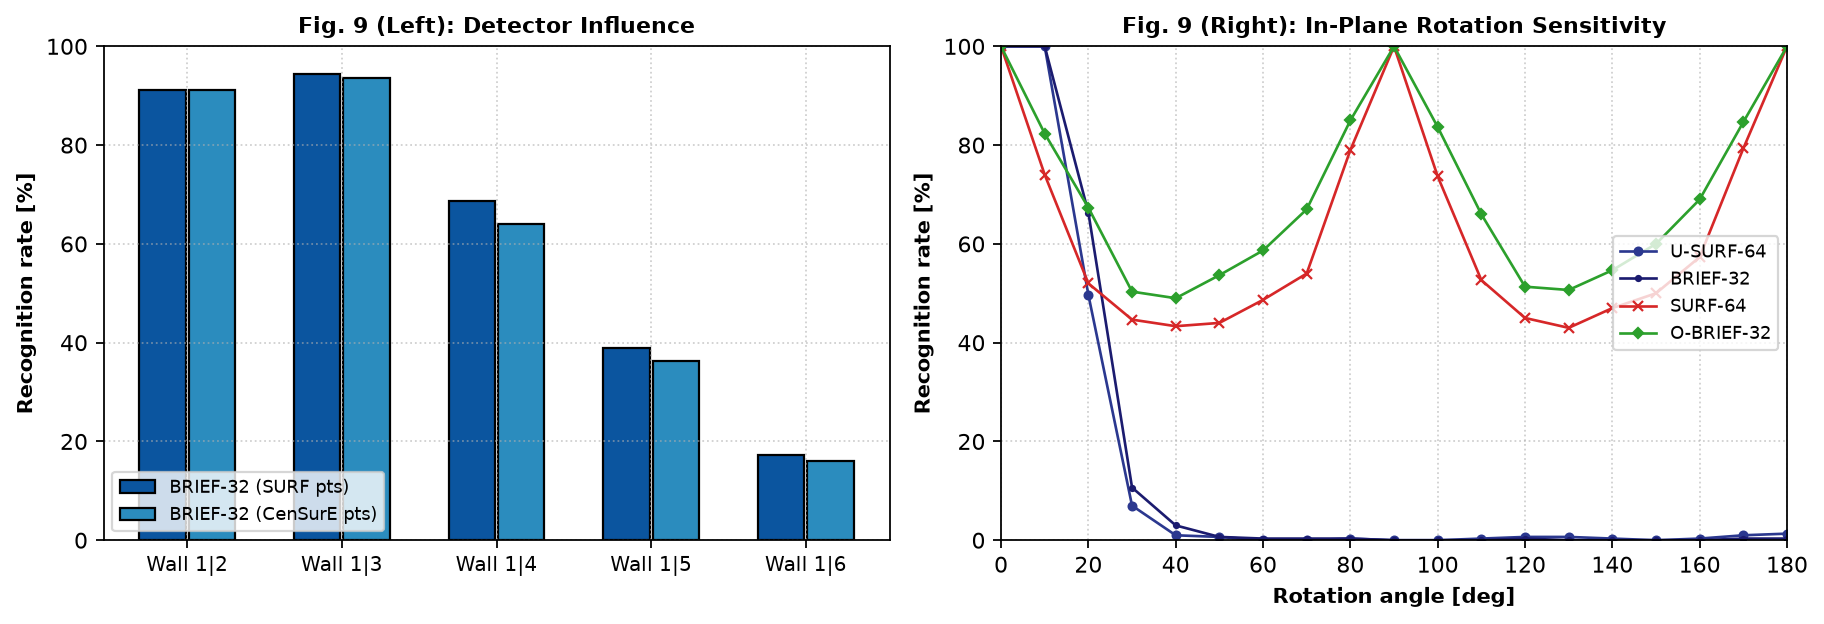
\includegraphics[width=\textwidth]{assets/fig9_rotation.png}
\end{column}
\begin{column}{0.43\textwidth}
\scriptsize
\textbf{Hallazgos experimentales (Fig. 9):}
\begin{enumerate}\setlength{\itemsep}{3pt}
    \item \textbf{Izquierda (CenSurE vs.\ SURF keypoints):} Combinar \texttt{BRIEF-32} con el detector rápido \textbf{CenSurE} no solo preserva la ventaja de velocidad total del pipeline, sino que \emph{supera ligeramente} el uso de keypoints SURF.
    \item \textbf{Derecha (Rotación $0^\circ$--$180^\circ$ en \texttt{Wall}):}
    \begin{itemize}\scriptsize\setlength{\itemsep}{2pt}
        \item Para rotaciones pequeñas ($0^\circ\text{--}15^\circ$), \textbf{BRIEF-32} y \textbf{U-SURF-64} superan a \textbf{SURF-64}.
        \item \textbf{O-BRIEF-32} (BRIEF rotado según la orientación estimada por SURF) se superpone casi perfectamente con \textbf{SURF-64}, probando que la pérdida de desempeño se debe a la incertidumbre del \emph{estimador de orientación}.
    \end{itemize}
\end{enumerate}
\end{column}
\end{columns}
\end{frame}

\begin{frame}{Comparación con Otros Métodos de Detección y Descripción}
\framesubtitle{Propiedades de invarianza, representación y complejidad}
\centering
\tiny
\renewcommand{\arraystretch}{1.28}
\setlength{\tabcolsep}{3.5pt}
\begin{tabular}{p{1.55cm}p{1.65cm}p{2.25cm}ccc p{1.55cm}}
\toprule
\textbf{Método} & \textbf{Detector Típico} & \textbf{Principio del Descriptor} & \textbf{Invar. Escala} & \textbf{Invar. Rotación} & \textbf{Métrica} & \textbf{Tamaño / Costo} \\
\midrule
\textbf{SIFT} \newline (Lowe, 2004) & DoG (Pirámide Gaussiana) & Histograma 3D de gradientes ($4\times4\times8$) & Sí & Sí (Histograma orientación) & Euclidiana ($L_2$) & 128 floats (512 B) \newline Costo Alto \\
\textbf{SURF-64} \newline (Bay et al., 2008) & Fast-Hessian (Im. Integrales) & Respuestas wavelet de Haar ($\sum d_x, \sum|d_x|$) & Sí & Sí (Ventana deslizante) & Euclidiana ($L_2$) & 64 floats (256 B) \newline Costo Medio \\
\textbf{U-SURF-64} \newline (Bay et al., 2008) & Fast-Hessian & Wavelets de Haar sin rotar (\emph{Upright}) & Sí & No (Tolera $\le 15^\circ$) & Euclidiana ($L_2$) & 64 floats (256 B) \newline Costo Medio \\
\textbf{BRIEF} \newline (Calonder, 2010) & FAST / CenSurE / SURF & Comparación binaria directa ($G_{II}$ Gaussiana) & \textbf{No} (Depende detector) & \textbf{No} (Tolera $\le 15^\circ$) & \textbf{Hamming} (\texttt{POPCNT}) & \textbf{16--64 B} \newline \textbf{Ultra-bajo} \\
\textbf{ORB} \newline (Rublee, 2011) & oFAST (Pirámide + Centroide) & \emph{Steered BRIEF} con pares descorrelacionados & Sí (Pirámide) & Sí (Momentos de intensidad) & Hamming (\texttt{POPCNT}) & 32 B \newline Muy bajo \\
\textbf{BRISK} \newline (Leutenegger, 2011) & AGAST multi-escala & Patrón circular concéntrico (pares cortos/largos) & Sí & Sí (Gradientes largos) & Hamming (\texttt{POPCNT}) & 64 B \newline Muy bajo \\
\bottomrule
\end{tabular}
\end{frame}


% ==============================================================================
% SECCIÓN 3: APPLICATIONS
% ==============================================================================
\section{Aplicaciones}

\begin{chapter}[assets/UNIbackground_negative]{sintefpurple}{3. Applications in Computer Vision}
\footnotesize
\begin{itemize}
    \item Dominios donde la restricción de orientación canónica se cumple naturalmente
    \item Sistemas de tiempo real, robótica móvil y dispositivos embebidos
    \item Indexación y reconstrucción 3D a gran escala
\end{itemize}
\end{chapter}

\footlinecolor{sintefpurple}
\footlinepayoff{Grupo 04 (FIIS-UNI) $\vert$ BRIEF (Calonder et al., ECCV 2010)}
% Slide 1
\begin{frame}{Aplicaciones Idóneas en Visión por Computadora}
\framesubtitle{¿Para qué problemas es más adecuado el descriptor BRIEF?}
\begin{columns}[T]
% --- Primera Columna ---
\begin{column}{0.48\textwidth}
\begin{colorblock}[black]{sintefgrey}{1. Sistemas SLAM Visual (Simultaneous Localization and Mapping)}
\scriptsize
\begin{itemize}\setlength{\itemsep}{2pt}
\item Utilizado en robótica y vehículos autónomos para el mapeo y localización en tiempo real donde la cámara se desplaza principalmente de forma frontal o lateral sin rotar sobre su eje.
\item La cámara captura video continuamente para construir un mapa del entorno y rastrear su propia trayectoria en tiempo real.
\end{itemize}
\end{colorblock}
\end{column}

% --- Segunda Columna ---
\begin{column}{0.48\textwidth}
\begin{figure}
    \centering
    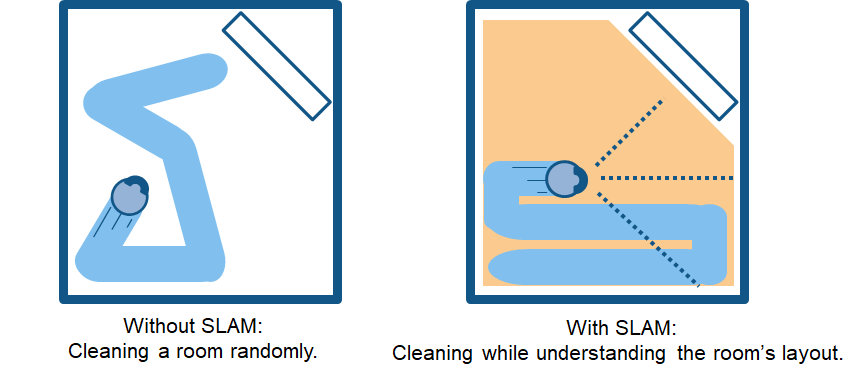
\includegraphics[width=\linewidth]{assets/slam.png}
    \caption{\scriptsize Representación de un sistema SLAM visual mapeando el entorno en tiempo real.}
\end{figure}
\end{column}

\end{columns}
\end{frame}

% Slide 2
\begin{frame}{Aplicaciones Idóneas en Visión por Computadora}
\framesubtitle{¿Para qué problemas es más adecuado el descriptor BRIEF?}
\begin{columns}[T]
% --- Primera Columna ---
\begin{column}{0.48\textwidth}
\begin{colorblock}[black]{sintefgrey}{2. Sistemas en tiempo real o embebidos}
\scriptsize
\begin{itemize}\setlength{\itemsep}{2pt}
\item Dado que los dispositivos móviles tienen restricciones severas de batería y procesamiento, BRIEF resulta ideal porque sus cadenas binarias se comparan mediante operaciones de hardware extremadamente ligeras: XOR seguido de un conteo de bits (popcount).

\item Por ejemplo, un descriptor SIFT típico requiere 512 bytes (128 flotantes). BRIEF suele requerir solo 16, 32 o 64 bytes (128, 256 o 512 bits) por punto de interés.
\end{itemize}
\end{colorblock}
\end{column}

% --- Segunda Columna ---
\begin{column}{0.48\textwidth}
\begin{colorblock}[black]{sintefgrey}{3. Reconstrucción e Indexación 3D Masiva}
\scriptsize
\begin{itemize}\setlength{\itemsep}{2pt}
    \item En la reconstrucción 3D el paso más costoso es encontrar qué puntos de una imagen coinciden con los de otra.
    \item Cuando la reconstrucción involucra miles de imágenes y millones de puntos 3D (nubes de puntos), la búsqueda lineal se vuelve imposible.
    \item A diferencia de SIFT o SURF (que usan vectores de números reales pesados), BRIEF convierte la información de un punto de interés en una cadena de bits (código binario).
\end{itemize}
\end{colorblock}
\end{column}

\end{columns}
\end{frame}
% Slide 3
\begin{frame}{Aplicaciones Idóneas en Visión por Computadora}
\framesubtitle{¿Para qué problemas es más adecuado el descriptor BRIEF?}
\begin{columns}[T]
% --- Primera Columna ---
\begin{column}{0.48\textwidth}
\begin{colorblock}[black]{sintefgrey}{4. Visión Estéreo Rectificada}
\scriptsize
\begin{itemize}\setlength{\itemsep}{2pt}
    \item En un sistema estéreo rectificado, se tienen dos cámaras alineadas de tal forma que sus planos de imagen son coplanares y sus ejes ópticos son paralelos.
    \item Al no haber rotación, el hecho de que BRIEF omita la corrección de orientación deja de ser una desventaja y se convierte en una ventaja táctica que ahorra tiempo de procesamiento.
\end{itemize}
\end{colorblock}
\end{column}

% --- Segunda Columna ---
\begin{column}{0.48\textwidth}
\begin{figure}
    \centering
    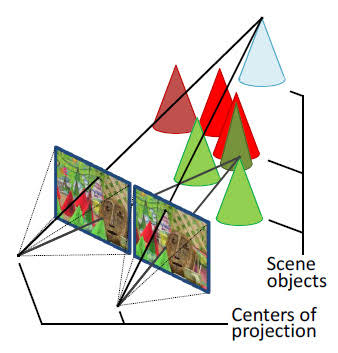
\includegraphics[width=\linewidth, height=0.65\textheight, keepaspectratio]{assets/stereo.jpeg}
    \caption{\scriptsize Visión Estéreo.}
\end{figure}
\end{column}

\end{columns}
\end{frame}
% ==============================================================================
% SECCIÓN 4: ADVANTAGES AND LIMITATIONS
% ==============================================================================
\section{Ventajas y limitaciones}

\begin{chapter}[assets/UNIbackground_negative]{sintefyellow}{4. Advantages and Limitations}
\footnotesize
\begin{itemize}
    \item Balance crítico entre eficiencia computacional e invarianza geométrica
    \item Fortalezas frente a métodos basados en gradientes flotantes
    \item Debilidades y evolución hacia descriptores binarios orientados
\end{itemize}
\end{chapter}

\footlinecolor{sintefyellow}
\footlinepayoff{Grupo 04 (FIIS-UNI) $\vert$ BRIEF (Calonder et al., ECCV 2010)}

\begin{frame}{Ventajas y Limitaciones del Método BRIEF}
\framesubtitle{Síntesis crítica de fortalezas y debilidades}
\begin{columns}[T]
\begin{column}{0.48\textwidth}
\begin{colorblock}[black]{sinteflightgreen}{Ventajas}
\scriptsize
\begin{enumerate}\setlength{\itemsep}{2.5pt}
    \item \textbf{Velocidad extrema de cómputo (35$\times$--41$\times$):} En la construcción del descriptor, dado que extrae el bitstring directamente mediante diferencias de intensidad sin calcular gradientes ni histogramas.
    \item \textbf{Emparejamiento por hardware ($\mathcal{O}(1)$ bitwise):}  Las comparaciones entre vectores binarios se realizan mediante la distancia de Hamming (operación \texttt{XOR} y conteo de bits \texttt{POPCNT}), la cual es considerablemente más veloz que las normas euclidianas.
    \item \textbf{Compacidad en memoria ($4\times$ a $16\times$ menor):} Con 16, 32 o 64 bytes supera a SURF (256 B) en secuencias sin rotación severa.
\end{enumerate}
\end{colorblock}
\end{column}
\begin{column}{0.48\textwidth}
\begin{colorblock}[black]{sintefgrey}{Limitaciones}
\scriptsize
\begin{enumerate}\setlength{\itemsep}{2.5pt}
    \item \textbf{Sensibilidad al ruido:} Se hace estrictamente necesario un paso de suavizado previo de la imagen.
    \item \textbf{Sensibilidad a rotaciones en plano ($>20^\circ$):} Falla catastróficamente si la cámara o el objeto rotan de manera significativa.
    \item \textbf{Sensibilidad a la escala:} No escala de forma nativa. Si un objeto se acerca o se aleja de la cámara, BRIEF suele fallar al emparejar los puntos clave.
    \item \textbf{Dependencia de un detector externo:} BRIEF es estrictamente un descriptor. No puede encontrar esquinas o puntos de interés por sí mismo; necesita trabajar junto a un detector como FAST o Harris.
\end{enumerate}
\end{colorblock}
\end{column}
\end{columns}
\end{frame}

\footlinecolor{}

\begin{frame}{Conclusiones y Legado Científico}
\framesubtitle{Impacto del trabajo de Calonder et al.\ en la Visión por Computadora moderna}
\scriptsize
\begin{itemize}\setlength{\itemsep}{3pt}
    \item \textbf{Cambio de paradigma métrico:} Desde un punto de vista teórico, BRIEF validó y consolidó la tendencia de abandonar la costosa métrica de distancia Euclidiana (norma $L_2$) para adoptar la distancia de Hamming en el emparejamiento de características locales.
    \item \textbf{Eliminación de la fase de entrenamiento:} A diferencia de trabajos previos que también usaban comparaciones de intensidad pero requerían entrenar árboles de clasificación o algoritmos bayesianos, BRIEF demostró que se podían generar firmas binarias directas y robustas sin ningún tipo de entrenamiento previo offline u online.
    \item \textbf{Pionero de la familia de descriptores binarios modernos:}
    \begin{itemize}\scriptsize
        \item \textbf{ORB} (Rublee et al., ICCV 2011): incorpora pirámide multi-escala FAST y orientación por centroide de intensidad (\emph{Steered BRIEF}) con aprendizaje de pares descorrelacionados (\emph{rBRIEF}).
        \item \textbf{BRISK} (Leutenegger et al., ICCV 2011) y \textbf{FREAK} (Alahi et al., CVPR 2012): extienden las comparaciones binarias de BRIEF a patrones circulares multi-escala.
    \end{itemize}
\end{itemize}

\vspace{0.1cm}
\begin{colorblock}[black]{sintefgrey}{Referencias Principales}
\tiny
\begin{enumerate}\setlength{\itemsep}{1pt}
    \item \textbf{Calonder, M., Lepetit, V., Strecha, C., \& Fua, P.} (2010). \emph{BRIEF: Binary Robust Independent Elementary Features}. In ECCV 2010 (pp.\ 778--792). Springer.
    \item \textbf{Bay, H., Ess, A., Tuytelaars, T., \& Van Gool, L.} (2008). \emph{SURF: Speeded Up Robust Features}. CVIU, 110(3), 346--359.
    \item \textbf{Lowe, D. G.} (2004). \emph{Distinctive Image Features from Scale-Invariant Keypoints}. IJCV, 60(2), 91--110.
    \item \textbf{Agrawal, M., Konolige, K., \& Blas, M. R.} (2008). \emph{CenSurE: Center Surround Extremas for Realtime Feature Detection and Matching}. In ECCV 2008.
    \item \textbf{Rublee, E., Rabaud, V., Konolige, K., \& Bradski, G.} (2011). \emph{ORB: An efficient alternative to SIFT or SURF}. In ICCV 2011.
\end{enumerate}
\end{colorblock}
\end{frame}

\backmatter
\end{document}
